\subsubsection{Adapted SAGAT}
\label{subsubsec:results_adapted_sagat_1}

For each question of the SAGAT questionnaire, the participant could score 1 point or a fraction of it. The closer to the value 1, higher is the situation awareness of the user. 

Figure \ref{fig:boxplot_sagat_blind_scene} brings the boxplot of the SAGAT score grouped by the guidance methods. It shows that the methods can be divided into two groups. The first one is composed of base, haptic belt and the mixture. This group received scores higher than the second group, composed of audio and virtual cane. Figure \ref{fig:boxplot_sagat_blind_rounds} shows the boxplot of the data grouped by round and confirms the general improvement of situation awareness from the first to the return round. 

\begin{figure}[!htb]
    \centering
    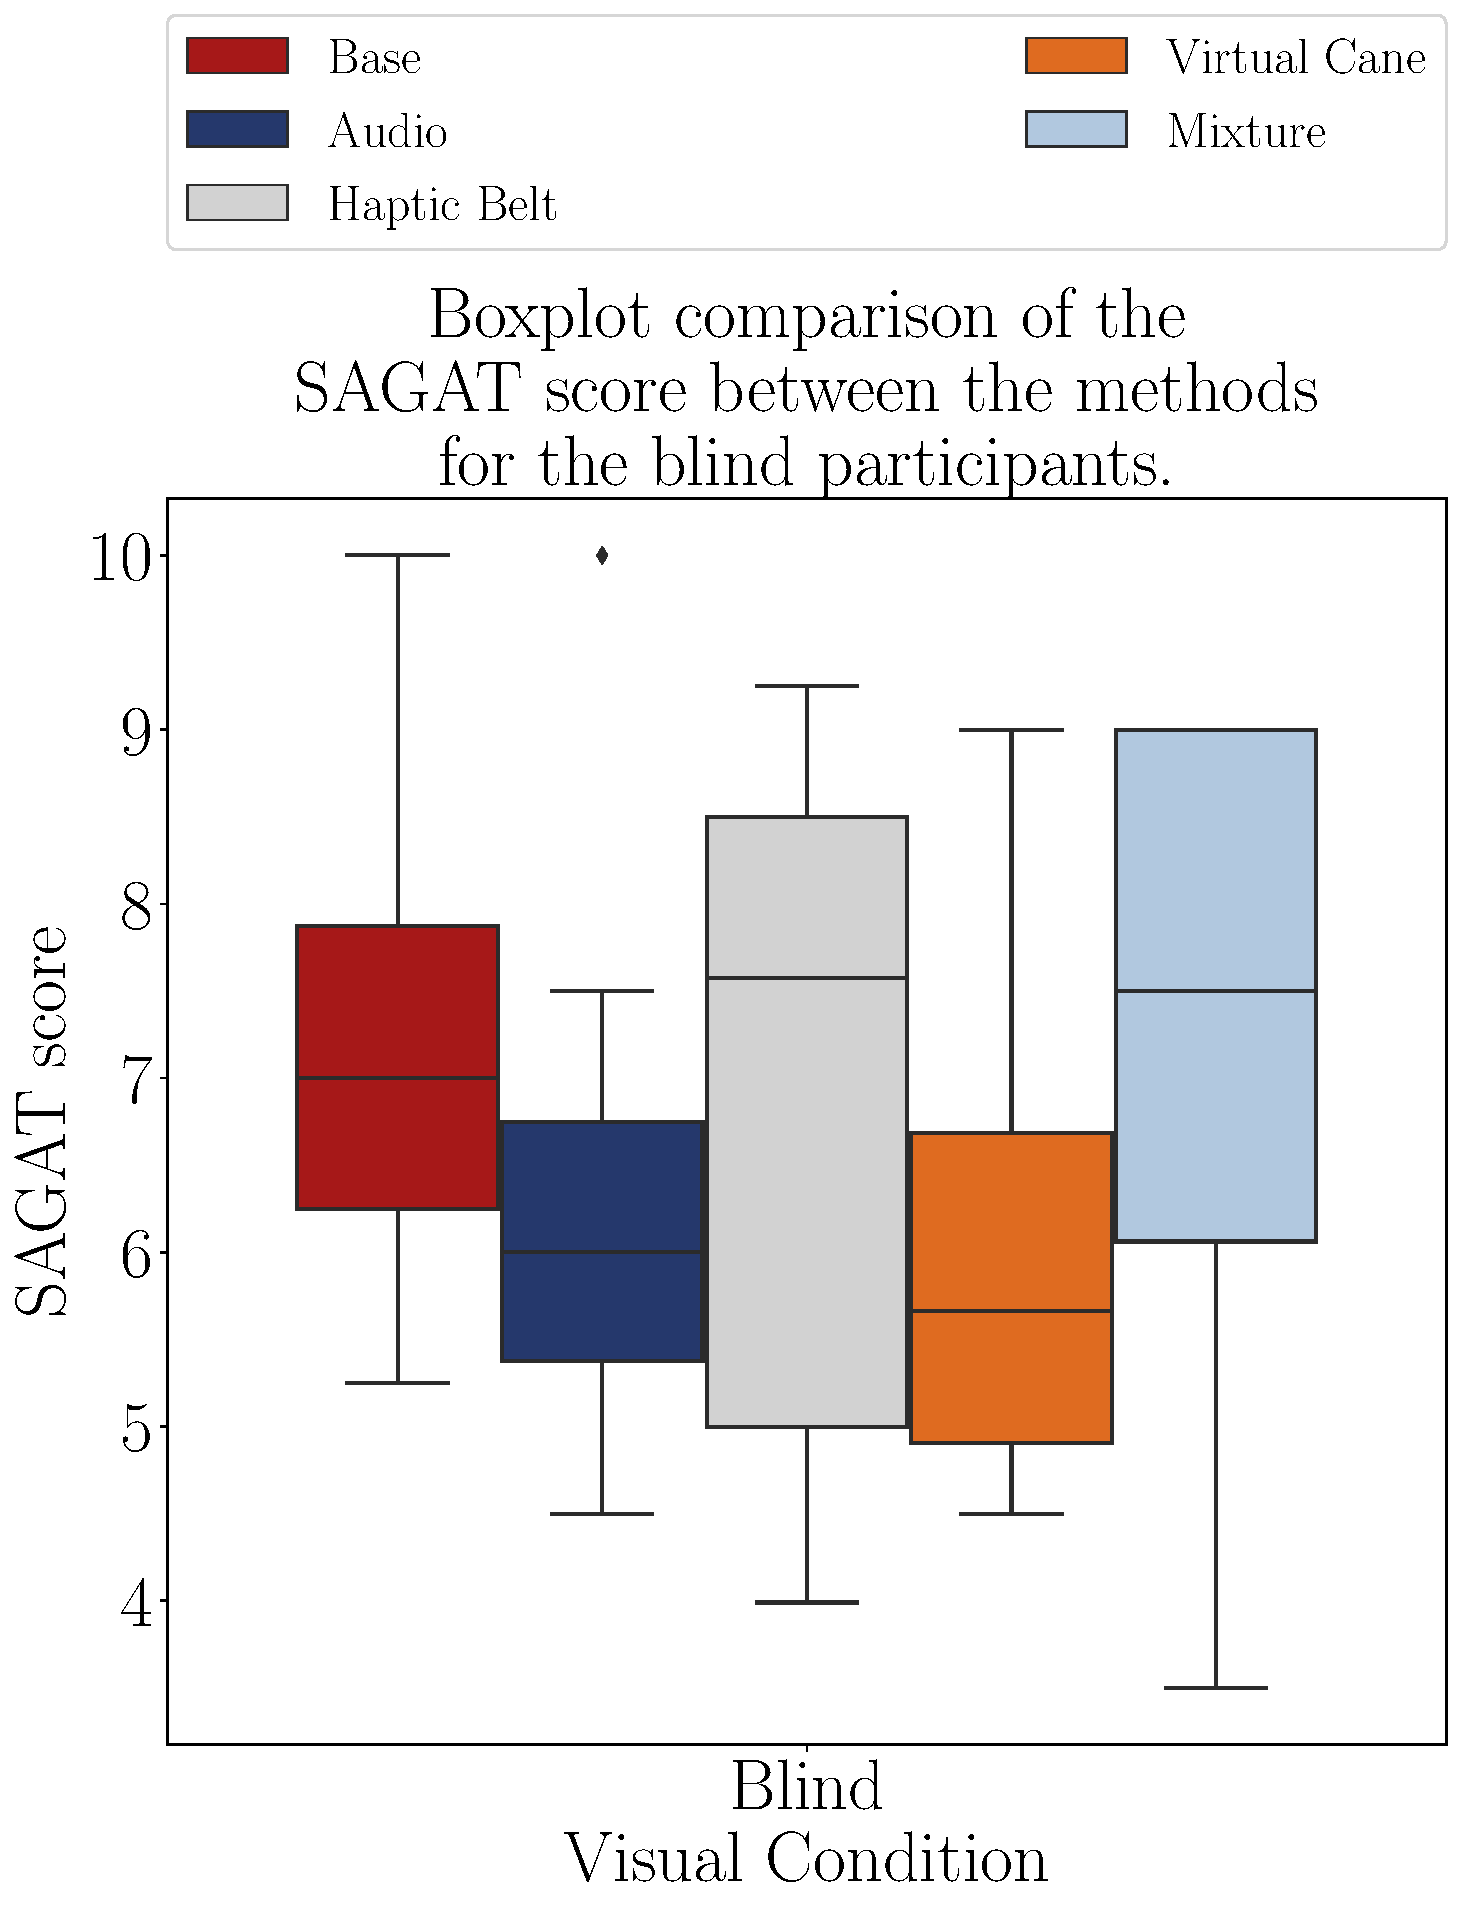
\includegraphics[width = 0.75\linewidth]{3 - Resultados/Figuras/boxplot_sagat_blind_scene.pdf}
    \caption{Boxplot of the SAGAT score of the blind participants grouped by the methods.}
    \label{fig:boxplot_sagat_blind_scene}
\end{figure}

\begin{figure}[!htb]
    \centering
    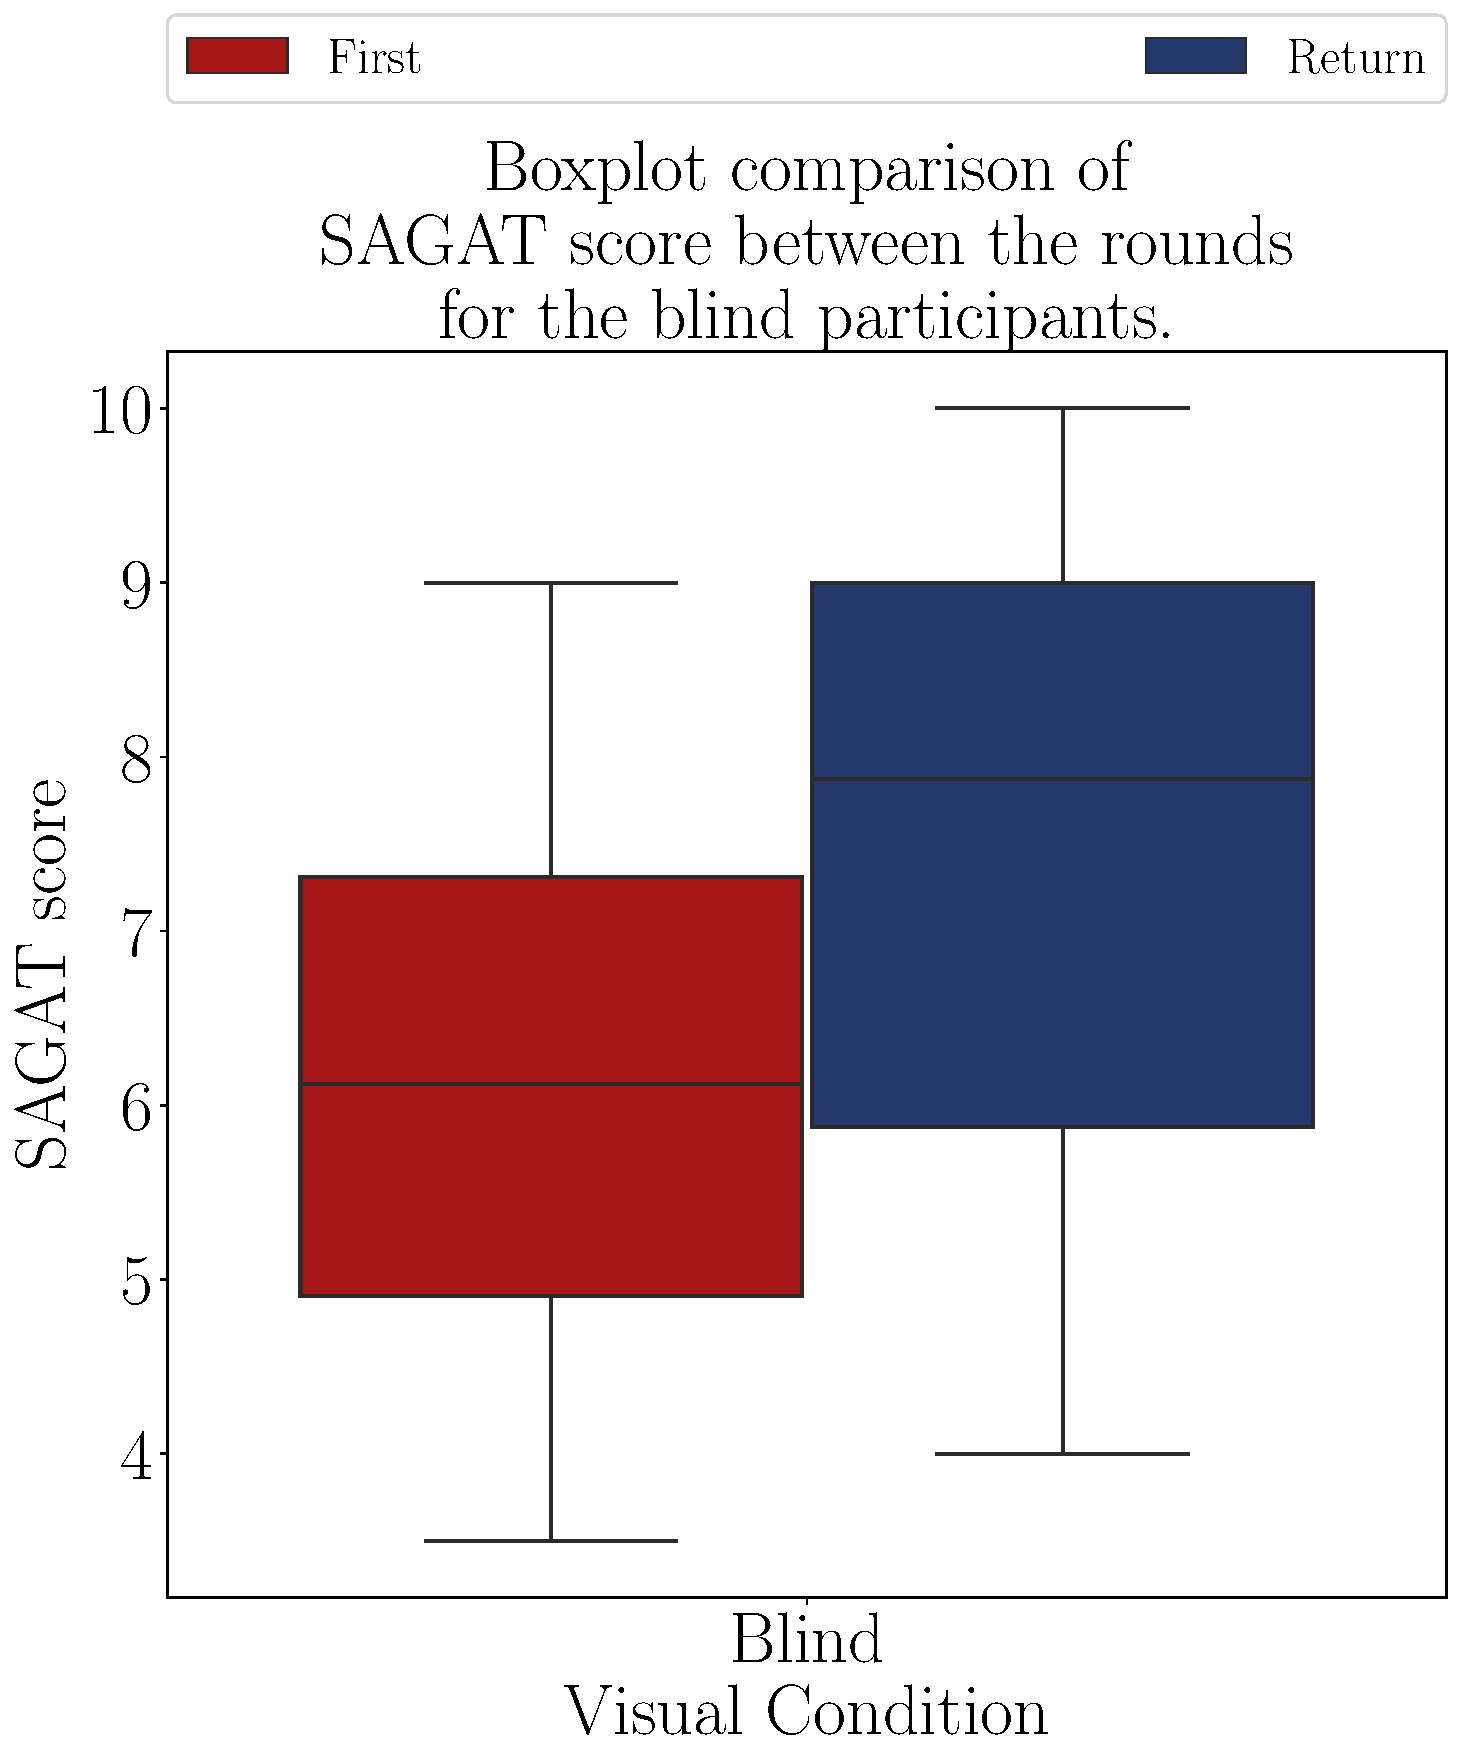
\includegraphics[width = 0.75\linewidth]{3 - Resultados/Figuras/boxplot_sagat_blind_rounds.pdf}
    \caption{Boxplot of the SAGAT score of the blind participants grouped by the rounds.}
    \label{fig:boxplot_sagat_blind_rounds}
\end{figure}

Table \ref{tab:blocanova_sagat_avg_two_way_blind} shows the ANOVA test p-value of the SAGAT score. It indicates that the round is a significant variable that influences the value of the SAGAT score. The same cannot be said for the method, which has no significant influence.


\begin{table}[!htb]
\centering
\caption{Anova p-value for the SAGAT score on each method for blinded users.}
\label{tab:blocanova_sagat_avg_two_way_blind}
\begin{tabular}{lrrrrr}
\toprule
          Source & P-Value \\
\midrule
    \    Methods &   0.277 \\
     \    Rounds & 0.002** \\
\    Interaction &   0.834 \\
\bottomrule
\end{tabular}
\end{table}

